\documentclass{standalone}
\usepackage{tikz}
\usetikzlibrary{patterns, positioning}


\begin{document}
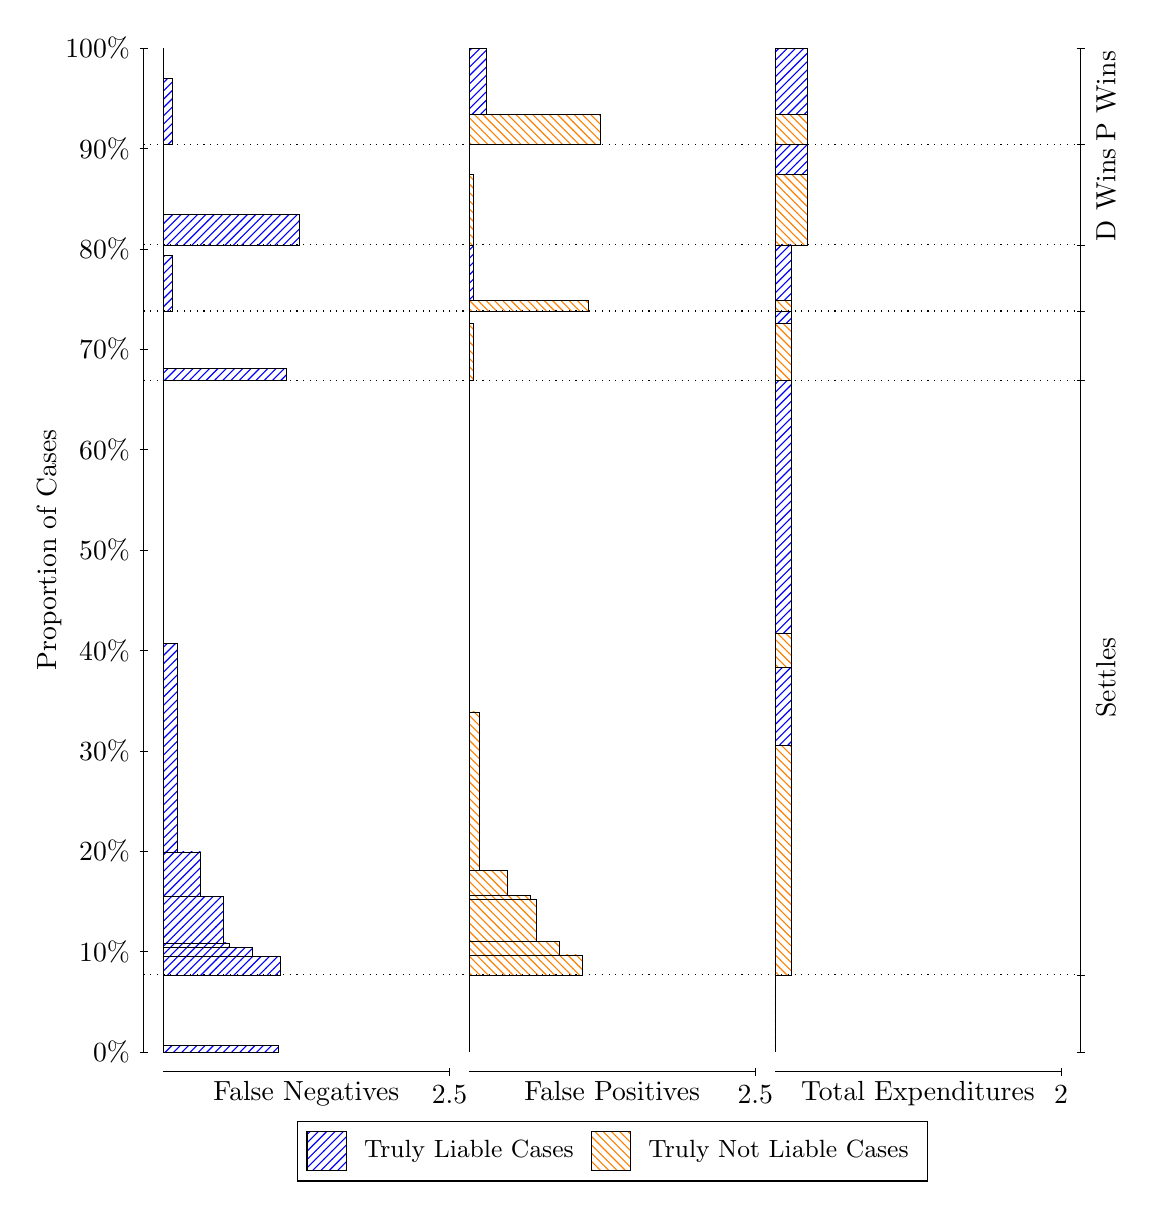
\begin{tikzpicture}
\draw[black, very thin] (1.5,1.75) -- (1.5,14.5);
\node[rotate=90, text=black, anchor=center] at (0.3, 8.125) {Proportion of Cases};
\draw[black, very thin] (1.45,1.75) -- (1.55,1.75);
\node[text=black, anchor=east] at (1.45, 1.75) {0\%};
\draw[black, very thin] (1.45,3.025) -- (1.55,3.025);
\node[text=black, anchor=east] at (1.45, 3.025) {10\%};
\draw[black, very thin] (1.45,4.3) -- (1.55,4.3);
\node[text=black, anchor=east] at (1.45, 4.3) {20\%};
\draw[black, very thin] (1.45,5.575) -- (1.55,5.575);
\node[text=black, anchor=east] at (1.45, 5.575) {30\%};
\draw[black, very thin] (1.45,6.85) -- (1.55,6.85);
\node[text=black, anchor=east] at (1.45, 6.85) {40\%};
\draw[black, very thin] (1.45,8.125) -- (1.55,8.125);
\node[text=black, anchor=east] at (1.45, 8.125) {50\%};
\draw[black, very thin] (1.45,9.4) -- (1.55,9.4);
\node[text=black, anchor=east] at (1.45, 9.4) {60\%};
\draw[black, very thin] (1.45,10.675) -- (1.55,10.675);
\node[text=black, anchor=east] at (1.45, 10.675) {70\%};
\draw[black, very thin] (1.45,11.95) -- (1.55,11.95);
\node[text=black, anchor=east] at (1.45, 11.95) {80\%};
\draw[black, very thin] (1.45,13.225) -- (1.55,13.225);
\node[text=black, anchor=east] at (1.45, 13.225) {90\%};
\draw[black, very thin] (1.45,14.5) -- (1.55,14.5);
\node[text=black, anchor=east] at (1.45, 14.5) {100\%};

\draw[black, very thin] (13.4,1.75) -- (13.4,14.5);
\draw[black, very thin] (13.35,1.75) -- (13.45,1.75);
\node[anchor=west] at (13.35, 1.75) {};
\draw[black, very thin] (13.35,2.7293) -- (13.45,2.7293);
\node[anchor=west] at (13.35, 2.7293) {};
\draw[black, very thin] (13.35,10.282) -- (13.45,10.282);
\node[anchor=west] at (13.35, 10.282) {};
\draw[black, very thin] (13.35,11.16) -- (13.45,11.16);
\node[anchor=west] at (13.35, 11.16) {};
\draw[black, very thin] (13.35,12) -- (13.45,12);
\node[anchor=west] at (13.35, 12) {};
\draw[black, very thin] (13.35,13.275) -- (13.45,13.275);
\node[anchor=west] at (13.35, 13.275) {};
\draw[black, very thin] (13.35,14.5) -- (13.45,14.5);
\node[anchor=west] at (13.35, 14.5) {};

\draw[black, very thin, pattern color=blue, pattern=north east lines] (1.75,1.75) rectangle (3.2033,1.8293);
\draw[black, very thin, pattern color=orange, pattern=north west lines] (1.75,1.8293) rectangle (1.75,2.7293);
\draw[black, very thin, pattern color=blue, pattern=north east lines] (1.75,2.7293) rectangle (3.2397,2.9625);
\draw[black, very thin, pattern color=blue, pattern=north east lines] (1.75,2.9625) rectangle (2.8763,3.0824);
\draw[black, very thin, pattern color=blue, pattern=north east lines] (1.75,3.0824) rectangle (2.5857,3.1345);
\draw[black, very thin, pattern color=blue, pattern=north east lines] (1.75,3.1345) rectangle (2.513,3.7222);
\draw[black, very thin, pattern color=blue, pattern=north east lines] (1.75,3.7222) rectangle (2.2223,4.2915);
\draw[black, very thin, pattern color=blue, pattern=north east lines] (1.75,4.2915) rectangle (1.9317,6.9429);
\draw[black, very thin, pattern color=orange, pattern=north west lines] (1.75,6.9429) rectangle (1.75,10.282);
\draw[black, very thin, pattern color=blue, pattern=north east lines] (1.75,10.282) rectangle (3.3123,10.436);
\draw[black, very thin, pattern color=orange, pattern=north west lines] (1.75,10.436) rectangle (1.75,11.16);
\draw[black, very thin, pattern color=blue, pattern=north east lines] (1.75,11.16) rectangle (1.859,11.863);
\draw[black, very thin, pattern color=orange, pattern=north west lines] (1.75,11.863) rectangle (1.75,12);
\draw[black, very thin, pattern color=blue, pattern=north east lines] (1.75,12) rectangle (3.4758,12.383);
\draw[black, very thin, pattern color=orange, pattern=north west lines] (1.75,12.383) rectangle (1.75,13.275);
\draw[black, very thin, pattern color=blue, pattern=north east lines] (1.75,13.275) rectangle (1.859,14.118);
\draw[black, very thin, pattern color=orange, pattern=north west lines] (1.75,14.118) rectangle (1.75,14.5);
\draw[black, very thin, pattern color=orange, pattern=north west lines] (5.6333,1.75) rectangle (5.6333,2.65);
\draw[black, very thin, pattern color=blue, pattern=north east lines] (5.6333,2.65) rectangle (5.6333,2.7293);
\draw[black, very thin, pattern color=orange, pattern=north west lines] (5.6333,2.7293) rectangle (7.0685,2.983);
\draw[black, very thin, pattern color=orange, pattern=north west lines] (5.6333,2.983) rectangle (6.7778,3.1572);
\draw[black, very thin, pattern color=orange, pattern=north west lines] (5.6333,3.1572) rectangle (6.4872,3.691);
\draw[black, very thin, pattern color=orange, pattern=north west lines] (5.6333,3.691) rectangle (6.4145,3.7393);
\draw[black, very thin, pattern color=orange, pattern=north west lines] (5.6333,3.7393) rectangle (6.1238,4.0572);
\draw[black, very thin, pattern color=orange, pattern=north west lines] (5.6333,4.0572) rectangle (5.7605,6.0684);
\draw[black, very thin, pattern color=blue, pattern=north east lines] (5.6333,6.0684) rectangle (5.6333,10.282);
\draw[black, very thin, pattern color=orange, pattern=north west lines] (5.6333,10.282) rectangle (5.6878,11.006);
\draw[black, very thin, pattern color=blue, pattern=north east lines] (5.6333,11.006) rectangle (5.6333,11.16);
\draw[black, very thin, pattern color=orange, pattern=north west lines] (5.6333,11.16) rectangle (7.1412,11.298);
\draw[black, very thin, pattern color=blue, pattern=north east lines] (5.6333,11.298) rectangle (5.6878,12);
\draw[black, very thin, pattern color=orange, pattern=north west lines] (5.6333,12) rectangle (5.6878,12.892);
\draw[black, very thin, pattern color=blue, pattern=north east lines] (5.6333,12.892) rectangle (5.6333,13.275);
\draw[black, very thin, pattern color=orange, pattern=north west lines] (5.6333,13.275) rectangle (7.3047,13.657);
\draw[black, very thin, pattern color=blue, pattern=north east lines] (5.6333,13.657) rectangle (5.8513,14.5);
\draw[black, very thin, pattern color=orange, pattern=north west lines] (9.5167,1.75) rectangle (9.5167,2.65);
\draw[black, very thin, pattern color=blue, pattern=north east lines] (9.5167,2.65) rectangle (9.5167,2.7293);
\draw[black, very thin, pattern color=orange, pattern=north west lines] (9.5167,2.7293) rectangle (9.721,5.6405);
\draw[black, very thin, pattern color=blue, pattern=north east lines] (9.5167,5.6405) rectangle (9.721,6.6334);
\draw[black, very thin, pattern color=orange, pattern=north west lines] (9.5167,6.6334) rectangle (9.721,7.0613);
\draw[black, very thin, pattern color=blue, pattern=north east lines] (9.5167,7.0613) rectangle (9.721,10.282);
\draw[black, very thin, pattern color=orange, pattern=north west lines] (9.5167,10.282) rectangle (9.721,11.006);
\draw[black, very thin, pattern color=blue, pattern=north east lines] (9.5167,11.006) rectangle (9.721,11.16);
\draw[black, very thin, pattern color=orange, pattern=north west lines] (9.5167,11.16) rectangle (9.721,11.298);
\draw[black, very thin, pattern color=blue, pattern=north east lines] (9.5167,11.298) rectangle (9.721,12);
\draw[black, very thin, pattern color=orange, pattern=north west lines] (9.5167,12) rectangle (9.9254,12.892);
\draw[black, very thin, pattern color=blue, pattern=north east lines] (9.5167,12.892) rectangle (9.9254,13.275);
\draw[black, very thin, pattern color=orange, pattern=north west lines] (9.5167,13.275) rectangle (9.9254,13.657);
\draw[black, very thin, pattern color=blue, pattern=north east lines] (9.5167,13.657) rectangle (9.9254,14.5);
\draw[black, dotted] (1.5,2.7293) -- (13.4,2.7293);
\draw[black, dotted] (1.5,10.282) -- (13.4,10.282);
\draw[black, dotted] (1.5,11.16) -- (13.4,11.16);
\draw[black, dotted] (1.5,12) -- (13.4,12);
\draw[black, dotted] (1.5,13.275) -- (13.4,13.275);
\draw[black, very thin] (1.75,1.5) -- (5.3833,1.5);
\node[text=black, anchor=north] at (3.5667, 1.5) {False Negatives};
\draw[black, very thin] (5.3833,1.45) -- (5.3833,1.55);
\node[text=black, anchor=north] at (5.3833, 1.45) {2.5};

\draw[black, very thin] (5.6333,1.5) -- (9.2667,1.5);
\node[text=black, anchor=north] at (7.45, 1.5) {False Positives};
\draw[black, very thin] (9.2667,1.45) -- (9.2667,1.55);
\node[text=black, anchor=north] at (9.2667, 1.45) {2.5};

\draw[black, very thin] (9.5167,1.5) -- (13.15,1.5);
\node[text=black, anchor=north] at (11.333, 1.5) {Total Expenditures};
\draw[black, very thin] (13.15,1.45) -- (13.15,1.55);
\node[text=black, anchor=north] at (13.15, 1.45) {2};


\node[text=black, centered, rotate=90] at (13.72, 6.5056) {Settles};


\node[text=black, centered, rotate=90] at (13.72, 12.638) {D Wins};
\node[text=black, centered, rotate=90] at (13.72, 13.887) {P Wins};

\draw (7.449999999999999,1.5) node[draw=none] (baseCoordinate) {};
\begin{scope}[align=center]
        \matrix[scale=0.5, draw=black, below=0.5cm of baseCoordinate, nodes={draw}, column sep=0.1cm]{
            \node[rectangle, draw, minimum width=0.5cm, minimum height=0.5cm, pattern color=blue, pattern=north east lines] {}; &
            \node[draw=none, font=\small, text=black] (B) {Truly Liable Cases}; &
            \node[rectangle, draw, minimum width=0.5cm, minimum height=0.5cm, pattern color=orange, pattern=north west lines] {}; &
            \node[draw=none, font=\small, text=black] (B) {Truly Not Liable Cases}; \\
            };
\end{scope}

\end{tikzpicture}
\end{document}